\begin{figure}[ht]
\centering
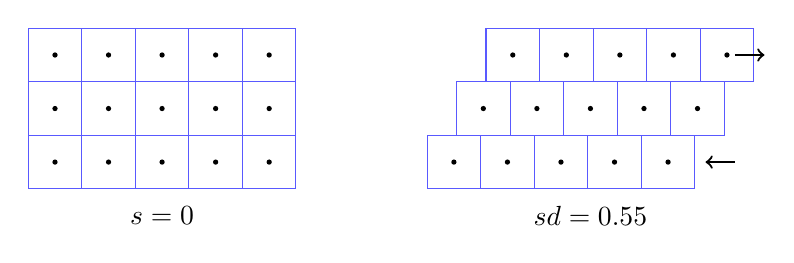
\begin{tikzpicture}[scale=.68]
 \begin{scope}
  \foreach \j in {-1,0,1} {
   \foreach \i in {-2,-1,0,1,2} {
    \draw[blue!65] (\i-.5,\j-.5) rectangle (\i+.5,\j+.5);
    \fill (\i,\j) circle (1.4pt);
   }
  }
  \node at (0,-2.0) {$s=0$};
 \end{scope}
 \begin{scope}[xshift=8cm]
  \foreach \j in {-1,0,1} {
   \foreach \i in {-2,-1,0,1,2} {
    \draw[blue!65] (\i+.55*\j-.5,\j-.5) rectangle (\i+.55*\j+.5,\j+.5);
    \fill (\i+.55*\j,\j) circle (1.4pt);
   }
  }
  \draw[->,thick] (2.7,1) -- (3.25,1);
  \draw[->,thick] (2.7,-1) -- (2.15,-1);
  \node at (0,-2.0) {$sd=0.55$};
 \end{scope}
\end{tikzpicture}
\caption{Sliding rows with $\tau=1$, after removing the common
translation. The tiles remain squares while row $j$ moves horizontally
by $sdj$. Each drawing shows a finite portion of a grid extending
infinitely in both directions. No gaps arise between the closed rows.}
\label{b:figure-rows}
\end{figure}
